\documentclass{standalone}
\usepackage{tikz}
\usetikzlibrary{patterns, positioning}


\begin{document}
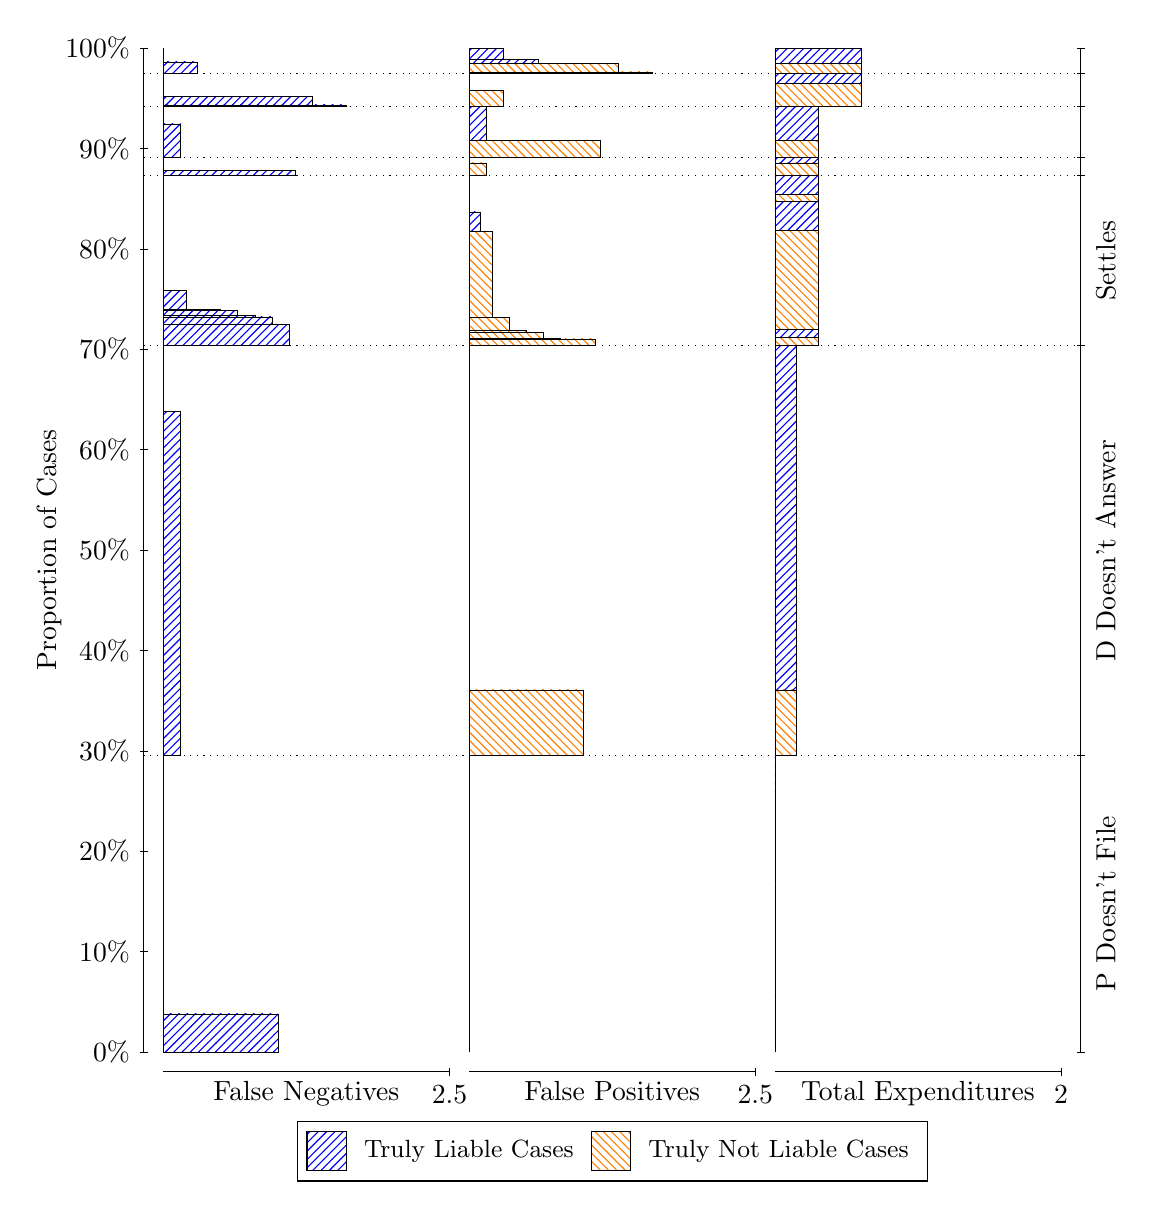
\begin{tikzpicture}
\draw[black, very thin] (1.5,1.75) -- (1.5,14.5);
\node[rotate=90, text=black, anchor=center] at (0.3, 8.125) {Proportion of Cases};
\draw[black, very thin] (1.45,1.75) -- (1.55,1.75);
\node[text=black, anchor=east] at (1.45, 1.75) {0\%};
\draw[black, very thin] (1.45,3.025) -- (1.55,3.025);
\node[text=black, anchor=east] at (1.45, 3.025) {10\%};
\draw[black, very thin] (1.45,4.3) -- (1.55,4.3);
\node[text=black, anchor=east] at (1.45, 4.3) {20\%};
\draw[black, very thin] (1.45,5.575) -- (1.55,5.575);
\node[text=black, anchor=east] at (1.45, 5.575) {30\%};
\draw[black, very thin] (1.45,6.85) -- (1.55,6.85);
\node[text=black, anchor=east] at (1.45, 6.85) {40\%};
\draw[black, very thin] (1.45,8.125) -- (1.55,8.125);
\node[text=black, anchor=east] at (1.45, 8.125) {50\%};
\draw[black, very thin] (1.45,9.4) -- (1.55,9.4);
\node[text=black, anchor=east] at (1.45, 9.4) {60\%};
\draw[black, very thin] (1.45,10.675) -- (1.55,10.675);
\node[text=black, anchor=east] at (1.45, 10.675) {70\%};
\draw[black, very thin] (1.45,11.95) -- (1.55,11.95);
\node[text=black, anchor=east] at (1.45, 11.95) {80\%};
\draw[black, very thin] (1.45,13.225) -- (1.55,13.225);
\node[text=black, anchor=east] at (1.45, 13.225) {90\%};
\draw[black, very thin] (1.45,14.5) -- (1.55,14.5);
\node[text=black, anchor=east] at (1.45, 14.5) {100\%};

\draw[black, very thin] (13.4,1.75) -- (13.4,14.5);
\draw[black, very thin] (13.35,1.75) -- (13.45,1.75);
\node[anchor=west] at (13.35, 1.75) {};
\draw[black, very thin] (13.35,5.5119) -- (13.45,5.5119);
\node[anchor=west] at (13.35, 5.5119) {};
\draw[black, very thin] (13.35,10.719) -- (13.45,10.719);
\node[anchor=west] at (13.35, 10.719) {};
\draw[black, very thin] (13.35,12.882) -- (13.45,12.882);
\node[anchor=west] at (13.35, 12.882) {};
\draw[black, very thin] (13.35,13.108) -- (13.45,13.108);
\node[anchor=west] at (13.35, 13.108) {};
\draw[black, very thin] (13.35,13.757) -- (13.45,13.757);
\node[anchor=west] at (13.35, 13.757) {};
\draw[black, very thin] (13.35,14.179) -- (13.45,14.179);
\node[anchor=west] at (13.35, 14.179) {};
\draw[black, very thin] (13.35,14.5) -- (13.45,14.5);
\node[anchor=west] at (13.35, 14.5) {};

\draw[black, very thin, pattern color=blue, pattern=north east lines] (1.75,1.75) rectangle (3.2033,2.2345);
\draw[black, very thin, pattern color=orange, pattern=north west lines] (1.75,2.2345) rectangle (1.75,5.5119);
\draw[black, very thin, pattern color=blue, pattern=north east lines] (1.75,5.5119) rectangle (1.968,9.8806);
\draw[black, very thin, pattern color=orange, pattern=north west lines] (1.75,9.8806) rectangle (1.75,10.719);
\draw[black, very thin, pattern color=blue, pattern=north east lines] (1.75,10.719) rectangle (3.3487,10.987);
\draw[black, very thin, pattern color=blue, pattern=north east lines] (1.75,10.987) rectangle (3.1307,11.086);
\draw[black, very thin, pattern color=blue, pattern=north east lines] (1.75,11.086) rectangle (2.9127,11.109);
\draw[black, very thin, pattern color=blue, pattern=north east lines] (1.75,11.109) rectangle (2.6947,11.167);
\draw[black, very thin, pattern color=blue, pattern=north east lines] (1.75,11.167) rectangle (2.4767,11.181);
\draw[black, very thin, pattern color=blue, pattern=north east lines] (1.75,11.181) rectangle (2.0407,11.426);
\draw[black, very thin, pattern color=orange, pattern=north west lines] (1.75,11.426) rectangle (1.75,12.882);
\draw[black, very thin, pattern color=blue, pattern=north east lines] (1.75,12.882) rectangle (3.4213,12.948);
\draw[black, very thin, pattern color=orange, pattern=north west lines] (1.75,12.948) rectangle (1.75,13.108);
\draw[black, very thin, pattern color=blue, pattern=north east lines] (1.75,13.108) rectangle (1.968,13.537);
\draw[black, very thin, pattern color=orange, pattern=north west lines] (1.75,13.537) rectangle (1.75,13.757);
\draw[black, very thin, pattern color=blue, pattern=north east lines] (1.75,13.757) rectangle (4.0753,13.778);
\draw[black, very thin, pattern color=blue, pattern=north east lines] (1.75,13.778) rectangle (3.6393,13.883);
\draw[black, very thin, pattern color=orange, pattern=north west lines] (1.75,13.883) rectangle (1.75,14.179);
\draw[black, very thin, pattern color=blue, pattern=north east lines] (1.75,14.179) rectangle (2.186,14.323);
\draw[black, very thin, pattern color=orange, pattern=north west lines] (1.75,14.323) rectangle (1.75,14.449);
\draw[black, very thin, pattern color=blue, pattern=north east lines] (1.75,14.449) rectangle (1.75,14.5);
\draw[black, very thin, pattern color=orange, pattern=north west lines] (5.6333,1.75) rectangle (5.6333,5.0274);
\draw[black, very thin, pattern color=blue, pattern=north east lines] (5.6333,5.0274) rectangle (5.6333,5.5119);
\draw[black, very thin, pattern color=orange, pattern=north west lines] (5.6333,5.5119) rectangle (7.0867,6.3499);
\draw[black, very thin, pattern color=blue, pattern=north east lines] (5.6333,6.3499) rectangle (5.6333,10.719);
\draw[black, very thin, pattern color=orange, pattern=north west lines] (5.6333,10.719) rectangle (7.232,10.805);
\draw[black, very thin, pattern color=orange, pattern=north west lines] (5.6333,10.805) rectangle (6.796,10.817);
\draw[black, very thin, pattern color=orange, pattern=north west lines] (5.6333,10.817) rectangle (6.578,10.887);
\draw[black, very thin, pattern color=orange, pattern=north west lines] (5.6333,10.887) rectangle (6.36,10.913);
\draw[black, very thin, pattern color=orange, pattern=north west lines] (5.6333,10.913) rectangle (6.142,11.081);
\draw[black, very thin, pattern color=orange, pattern=north west lines] (5.6333,11.081) rectangle (5.924,12.175);
\draw[black, very thin, pattern color=blue, pattern=north east lines] (5.6333,12.175) rectangle (5.7787,12.42);
\draw[black, very thin, pattern color=blue, pattern=north east lines] (5.6333,12.42) rectangle (5.6333,12.882);
\draw[black, very thin, pattern color=orange, pattern=north west lines] (5.6333,12.882) rectangle (5.8513,13.042);
\draw[black, very thin, pattern color=blue, pattern=north east lines] (5.6333,13.042) rectangle (5.6333,13.108);
\draw[black, very thin, pattern color=orange, pattern=north west lines] (5.6333,13.108) rectangle (7.3047,13.328);
\draw[black, very thin, pattern color=blue, pattern=north east lines] (5.6333,13.328) rectangle (5.8513,13.757);
\draw[black, very thin, pattern color=orange, pattern=north west lines] (5.6333,13.757) rectangle (6.0693,13.96);
\draw[black, very thin, pattern color=orange, pattern=north west lines] (5.6333,13.96) rectangle (5.6333,14.054);
\draw[black, very thin, pattern color=blue, pattern=north east lines] (5.6333,14.054) rectangle (5.6333,14.179);
\draw[black, very thin, pattern color=orange, pattern=north west lines] (5.6333,14.179) rectangle (7.9587,14.196);
\draw[black, very thin, pattern color=orange, pattern=north west lines] (5.6333,14.196) rectangle (7.5227,14.305);
\draw[black, very thin, pattern color=blue, pattern=north east lines] (5.6333,14.305) rectangle (6.5053,14.356);
\draw[black, very thin, pattern color=blue, pattern=north east lines] (5.6333,14.356) rectangle (6.0693,14.5);
\draw[black, very thin, pattern color=orange, pattern=north west lines] (9.5167,1.75) rectangle (9.5167,5.0274);
\draw[black, very thin, pattern color=blue, pattern=north east lines] (9.5167,5.0274) rectangle (9.5167,5.5119);
\draw[black, very thin, pattern color=orange, pattern=north west lines] (9.5167,5.5119) rectangle (9.7892,6.3499);
\draw[black, very thin, pattern color=blue, pattern=north east lines] (9.5167,6.3499) rectangle (9.7892,10.719);
\draw[black, very thin, pattern color=orange, pattern=north west lines] (9.5167,10.719) rectangle (10.062,10.827);
\draw[black, very thin, pattern color=blue, pattern=north east lines] (9.5167,10.827) rectangle (10.062,10.922);
\draw[black, very thin, pattern color=orange, pattern=north west lines] (9.5167,10.922) rectangle (10.062,12.185);
\draw[black, very thin, pattern color=blue, pattern=north east lines] (9.5167,12.185) rectangle (10.062,12.552);
\draw[black, very thin, pattern color=orange, pattern=north west lines] (9.5167,12.552) rectangle (10.062,12.638);
\draw[black, very thin, pattern color=blue, pattern=north east lines] (9.5167,12.638) rectangle (10.062,12.882);
\draw[black, very thin, pattern color=orange, pattern=north west lines] (9.5167,12.882) rectangle (10.062,13.042);
\draw[black, very thin, pattern color=blue, pattern=north east lines] (9.5167,13.042) rectangle (10.062,13.108);
\draw[black, very thin, pattern color=orange, pattern=north west lines] (9.5167,13.108) rectangle (10.062,13.328);
\draw[black, very thin, pattern color=blue, pattern=north east lines] (9.5167,13.328) rectangle (10.062,13.757);
\draw[black, very thin, pattern color=orange, pattern=north west lines] (9.5167,13.757) rectangle (10.607,14.054);
\draw[black, very thin, pattern color=blue, pattern=north east lines] (9.5167,14.054) rectangle (10.607,14.179);
\draw[black, very thin, pattern color=orange, pattern=north west lines] (9.5167,14.179) rectangle (10.607,14.305);
\draw[black, very thin, pattern color=blue, pattern=north east lines] (9.5167,14.305) rectangle (10.607,14.5);
\draw[black, dotted] (1.5,5.5119) -- (13.4,5.5119);
\draw[black, dotted] (1.5,10.719) -- (13.4,10.719);
\draw[black, dotted] (1.5,12.882) -- (13.4,12.882);
\draw[black, dotted] (1.5,13.108) -- (13.4,13.108);
\draw[black, dotted] (1.5,13.757) -- (13.4,13.757);
\draw[black, dotted] (1.5,14.179) -- (13.4,14.179);
\draw[black, very thin] (1.75,1.5) -- (5.3833,1.5);
\node[text=black, anchor=north] at (3.5667, 1.5) {False Negatives};
\draw[black, very thin] (5.3833,1.45) -- (5.3833,1.55);
\node[text=black, anchor=north] at (5.3833, 1.45) {2.5};

\draw[black, very thin] (5.6333,1.5) -- (9.2667,1.5);
\node[text=black, anchor=north] at (7.45, 1.5) {False Positives};
\draw[black, very thin] (9.2667,1.45) -- (9.2667,1.55);
\node[text=black, anchor=north] at (9.2667, 1.45) {2.5};

\draw[black, very thin] (9.5167,1.5) -- (13.15,1.5);
\node[text=black, anchor=north] at (11.333, 1.5) {Total Expenditures};
\draw[black, very thin] (13.15,1.45) -- (13.15,1.55);
\node[text=black, anchor=north] at (13.15, 1.45) {2};

\node[text=black, centered, rotate=90] at (13.72, 3.6309) {P Doesn't File};
\node[text=black, centered, rotate=90] at (13.72, 8.1152) {D Doesn't Answer};
\node[text=black, centered, rotate=90] at (13.72, 11.8) {Settles};





\draw (7.449999999999999,1.5) node[draw=none] (baseCoordinate) {};
\begin{scope}[align=center]
        \matrix[scale=0.5, draw=black, below=0.5cm of baseCoordinate, nodes={draw}, column sep=0.1cm]{
            \node[rectangle, draw, minimum width=0.5cm, minimum height=0.5cm, pattern color=blue, pattern=north east lines] {}; &
            \node[draw=none, font=\small, text=black] (B) {Truly Liable Cases}; &
            \node[rectangle, draw, minimum width=0.5cm, minimum height=0.5cm, pattern color=orange, pattern=north west lines] {}; &
            \node[draw=none, font=\small, text=black] (B) {Truly Not Liable Cases}; \\
            };
\end{scope}

\end{tikzpicture}
\end{document}